\documentclass[12pt]{article}

\usepackage{graphicx}
\usepackage{paralist}
\usepackage{amsfonts}
\usepackage{amsmath}
\usepackage{hhline}
\usepackage{booktabs}
\usepackage{multirow}
\usepackage{multicol}
\usepackage{url}

\oddsidemargin -10mm
\evensidemargin -10mm
\textwidth 160mm
\textheight 200mm
\renewcommand\baselinestretch{1.0}

\pagestyle {plain}
\pagenumbering{arabic}

\newcounter{stepnum}

%% Comments

\usepackage{color}

\newif\ifcomments\commentstrue

\ifcomments
\newcommand{\authornote}[3]{\textcolor{#1}{[#3 ---#2]}}
\newcommand{\todo}[1]{\textcolor{red}{[TODO: #1]}}
\else
\newcommand{\authornote}[3]{}
\newcommand{\todo}[1]{}
\fi

\newcommand{\wss}[1]{\authornote{blue}{SS}{#1}}

\title{Assignment 4, Design Specification}
\author{SFWRENG 2AA4}

\begin{document}

\maketitle
This Module Interface Specification (MIS) document contains modules, types and
methods for implementing the game \textit{2048}. At the start of the game, there are two numbers displayed on the Board usually randomized between 2 and 4, then the user can perform some operations via up/down/left or right arrow key in order to achieve a tile containing 2048.\\\\ The game works on the principle that every time  a tile is moved, another tile pops up in a random manner anywhere on the board, when two tiles with the same number on them collide with one another as they are moved, they will merge into one tile with the sum of the numbers written on them initially. The target is always to make a tile having 2048 but if the user wants the game can be continued even after achieving 2048 on any tile.\\\\ The 
game can be launched and played by typing \texttt{make game} on Virtual Machine. The test cases could be run by typing \texttt{make test} on Virtual Machine.\\
\graphicspath{ {/Users/karansingh/Desktop} }
\begin{center}
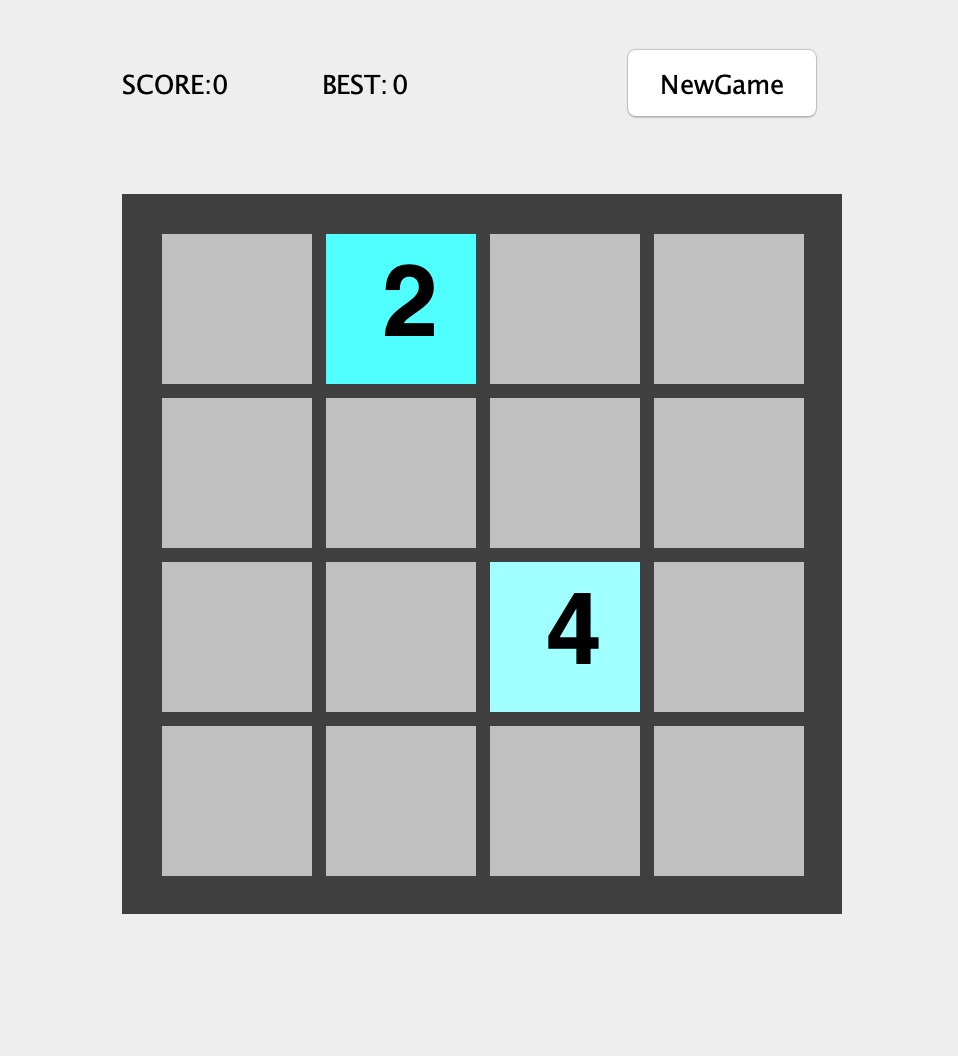
\includegraphics[width=6cm, height=6cm]{img.png}
\end{center}
\newpage

\section* {GUI Module}

\subsection*{Module}

GUI Module

\subsection* {Uses}

JPanel\\
KeyListener\\
ActionListener\\

\subsection* {Syntax}

\subsubsection* {Exported Constants}

None

\subsubsection* {Exported Types}

None


\subsubsection* {Exported Access Programs}

\begin{tabular}{| l | l | l | p{6cm} |}
\hline
\textbf{Routine name} & \textbf{In} & \textbf{Out} & \textbf{Exceptions}\\
\hline
new GUI & & self& \\
\hline
TextOnSquare & $\mathbb{N}$ &  & \\
\hline
startgame & GameCal &  & \\
\hline
keyTyped & KeyEvent &  & \\
\hline
keyPressed & KeyEvent & & \\
\hline
keyReleased & KeyEvent &  & \\
\hline
actionPerformed & ActionEvent & & \\
\hline
\end{tabular}

\subsection* {Semantics}

\subsection* {State Variables}

gameover: $\mathbb{N}$ \\
frame: JFrame\\
calc: GameCal \\
score: JLabel\\
best: JLabel\\
completed: JLabel\\ 
newgame: JButton\\
b: seq [$\mathbb{N}$,$\mathbb{N}$] of JLabel

\subsection* {State Invariant}

None

\subsection*{Assumptions}

None

\subsection* {Access Routine Semantics}

new GUI():

\begin{itemize}
  \item output: out $:=$ self
  \item transition $:=$   \begin{tabular}{| l | l |}
  \hline
  ~ & $:=$ \\
  \hline
  b & new JLabel[4][4] \\
  \hline
  frame & new JFrame() \\
  \hline
  completed & new JLabel() \\
  \hline
  score & new JLabel() \\
  \hline
  best & new JLabel() \\
  \hline
  newGame & new JButton \\
  \hline
  $y\_coordinate$ & 20 \\
  \hline
  $x\_coordinate$ & 20 \\
  \hline
  \end{tabular}\\\\
  All the display components of GUI can be edited using in-built functions like .setBounds, .setBackground or .setOpaque etc.
   \item exception $:=$ None
  \end{itemize}
\newpage
\noindent TextOnSquare(value, i , j):

\begin{itemize}
  \item transition $:=$ checks for the length of the digits in the tile and depending upon their lengths their font sizes are selected to fit them in the tile. For different values color are chosen by the log function imported via math library.\\\\
  \medskip
  \begin{tabular}{| l | l |}
  \hline
  \textbf{length of the digit} & Font Size \\
  \hline
  value.length $==$ 1 &  20 \\
  \hline
  value.length $==$ 2 &  20 \\
  \hline
  value.length $==$ 3 & 20 \\
  \hline
  value.length $==$ 4 & 20 \\
  \hline
  value.length $==$ 5 & 20 \\
  \hline
  \end{tabular}
    \item output: out $:=$ None
  \item exception $:=$ None
\end{itemize}

\noindent startgame(GameCal c):
\begin{itemize}
\item transition: calc $:=$ c
  \item output:$out$ $:=$ None
  \item exception $:=$ None
\end{itemize}

\noindent keyTyped(KeyEvent e): \textit{//overriden function}

\begin{itemize}
\item transition $:=$ None
  \item output:$out$ $:=$ None
  \item exception $:=$ None
\end{itemize}

\noindent keyPressed(KeyEvent e): \textit{//overriden function}

\begin{itemize}
\item transition $:=$ checks which key is pressed from the keyboard out of 'w','s','a' and 'd'. \textit{//w is for up , s is for down , a is for left and d is for right.}
  \item output:$out$ $:=$ None
  \item exception $:=$ None
\end{itemize}

\noindent keyReleased(KeyEvent e): \textit{//overriden function}

\begin{itemize}
\item transition $:=$ None
  \item output:$out$ $:=$ None
  \item exception $:=$ None
\end{itemize}

\noindent actionPerformed(ActionEvent e): \textit{//overriden function}

\begin{itemize}
\item transition $:=$ spawns a 2 or a 4 when a new game is started or whenever a directional key is pressed. 
  \item output:$out$ $:=$ None
  \item exception $:=$ None
\end{itemize}
\newpage

\section* {GameCal Module}

\subsection* {Module}

GameCal

\subsection*{Uses}

None

\subsection* {Syntax}

\subsection*{Exported Constants}

None

\subsection*{Exported Types}

None

\subsubsection* {Exported Access Programs}

\begin{tabular}{| l | l | l | p{6cm} |}
\hline
\textbf{Routine name} & \textbf{In} & \textbf{Out} & \textbf{Exceptions}\\
\hline
GameCal & & new GameCal& \\
\hline
getResult &  & $\mathbb{N}$ & \\
\hline
spawn &  &  & \\
\hline
getMaxOnSquare &  & $\mathbb{N}$ & \\
\hline
newGameStart &  & & \\
\hline
allSquareFull &  & $\mathbb{B}$ & \\
\hline
gameCompleted &  & $\mathbb{B}$ & \\
\hline
up &  &  & \\
\hline
down &  &  & \\
\hline
left &  &  & \\
\hline
right &  &  & \\
\hline
verticalMove & $\mathbb{N}$,$\mathbb{N}$,String  &  & \\
\hline
horizontalMove & $\mathbb{N}$,$\mathbb{N}$,String &  & \\
\hline
\end{tabular}

\subsection*{State Variables}

boundry: $\mathbb{N}$ \\
result: $\mathbb{N}$ 

\subsection*{State Invariant}

None

\subsection*{Assumptions}

None

\subsubsection* {Access Routine Semantics}

new GameCal():

\begin{itemize}
  \item output: out $:=$ self
  \item transition : boundry, result $:=$ 0, 0
    \item exception $:=$ None
\end{itemize}

\noindent getResult():
\begin{itemize}
   \item transition $:=$ None
     \item output: out $:=$ result
       \item exception $:=$ None
       \end{itemize}
       
\noindent spawn():
\begin{itemize}
   \item transition $:=$ spawns a 2 or a 4 at an empty tile whenever a move is made or whenever it is clicked on new game.\\
   x $<$ 0.1 $\implies$ a 4 will be spawn $||$ x $\ge$ 0.1 $\implies$ 2 will be spawn
     \item output: out $:=$ None
       \item exception $:=$ None
       \end{itemize}
       
\noindent newGameStart():
\begin{itemize}
   \item transition $:=$ refreshes the game everytime it is clicked on new game
     \item output: out $:=$ None
       \item exception $:=$ None
       \end{itemize}

\noindent allSquareFull():
\begin{itemize}
\item transition: count $:=$ 0
  \item output:$out$ $:=$ returns true when all the tiles are filled and there is no move possible and false otherwise.
      \item exception $:=$ None
\end{itemize}

\noindent gameCompleted():
\begin{itemize}
\item transition: count $:=$ 0\\
 checks if there is a move possible among any row or column corresponding to a particular tile. 
  \item output:$out$ $:=$ returns true when any of the tile reaches 2048 and false otherwise.
      \item exception $:=$ None
\end{itemize}

\noindent up():
\begin{itemize}
\item transition: boundry $:=$ 0\\
 checks if there is a move possible among any row particularly in up direction . Stops responding when the
 value or the tile is in the top most row that is the 0th row.
  \item output:$out$ $:=$ None
      \item exception $:=$ None
\end{itemize}

\noindent down():
\begin{itemize}
\item transition: boundry $:=$ 3\\
 checks if there is a move possible among any row particularly in down direction . Stops responding when the
 value or the tile is in the bottom most row that is the 3rd row.
  \item output:$out$ $:=$ None
      \item exception $:=$ None
\end{itemize}

\noindent left():
\begin{itemize}
\item transition: boundry $:=$ 0\\
 checks if there is a move possible among any column particularly in left direction . Stops responding when the value or the tile is in the left most column that is the 0th column.
  \item output:$out$ $:=$ None
      \item exception $:=$ None
\end{itemize}

\noindent right():
\begin{itemize}
\item transition: boundry $:=$ 3\\
 checks if there is a move possible among any column particularly in right direction. Stops responding when the value or the tile is in the right most column that is the 3rd column.
  \item output:$out$ $:=$ None
      \item exception $:=$ None
\end{itemize}

\noindent verticalMove(row,col,direction):
\begin{itemize}
\item transition $:=$ None\\
Compares two tile's values together and if they are the same or if one is equal to 0 (plain tile) - their values are added (provided that the tiles we are comparing are two different tiles and they are moving towards the appropriate direction),this is done through the entire column.
  \item output:$out$ $:=$ None
      \item exception $:=$ None
\end{itemize}

\noindent horizontalMove(row,col,direction):
\begin{itemize}
\item transition: boundry $:=$ 3\\
Compares two tile's values together and if they are the same or if one is equal to 0 (plain tile) - their values are added (provided that the tiles we are comparing are two different tiles and they are moving towards the appropriate direction) ,this is done through the entire row.
  \item output:$out$ $:=$ None
      \item exception $:=$ None
\end{itemize}

\newpage

\section*{Critique of Design}

\begin{itemize}
  \item I did not make my GameCal as an ADT module as I thought it could be a little time consuming and complicated to implement although it can be more convenient in terms of essentiality. 
  
  \item Once the game is played and a best is stored it refreshes when the function is run again although its data could have been stored to give it a moe lively look, but just to save time it as avoided in this specification.
  \item In the GameCal Module there is function named $getMaxOnSquare()$ although it could have been avoided but it was made in this specification test some edge cases .
  \item This specification might not be as efficient as it could be because there are certain conditions in the GameCal module that are complicated and might take a little longer time than usual.
  
  
\end{itemize}

\noindent UML diagram for modules of Assignment 3:

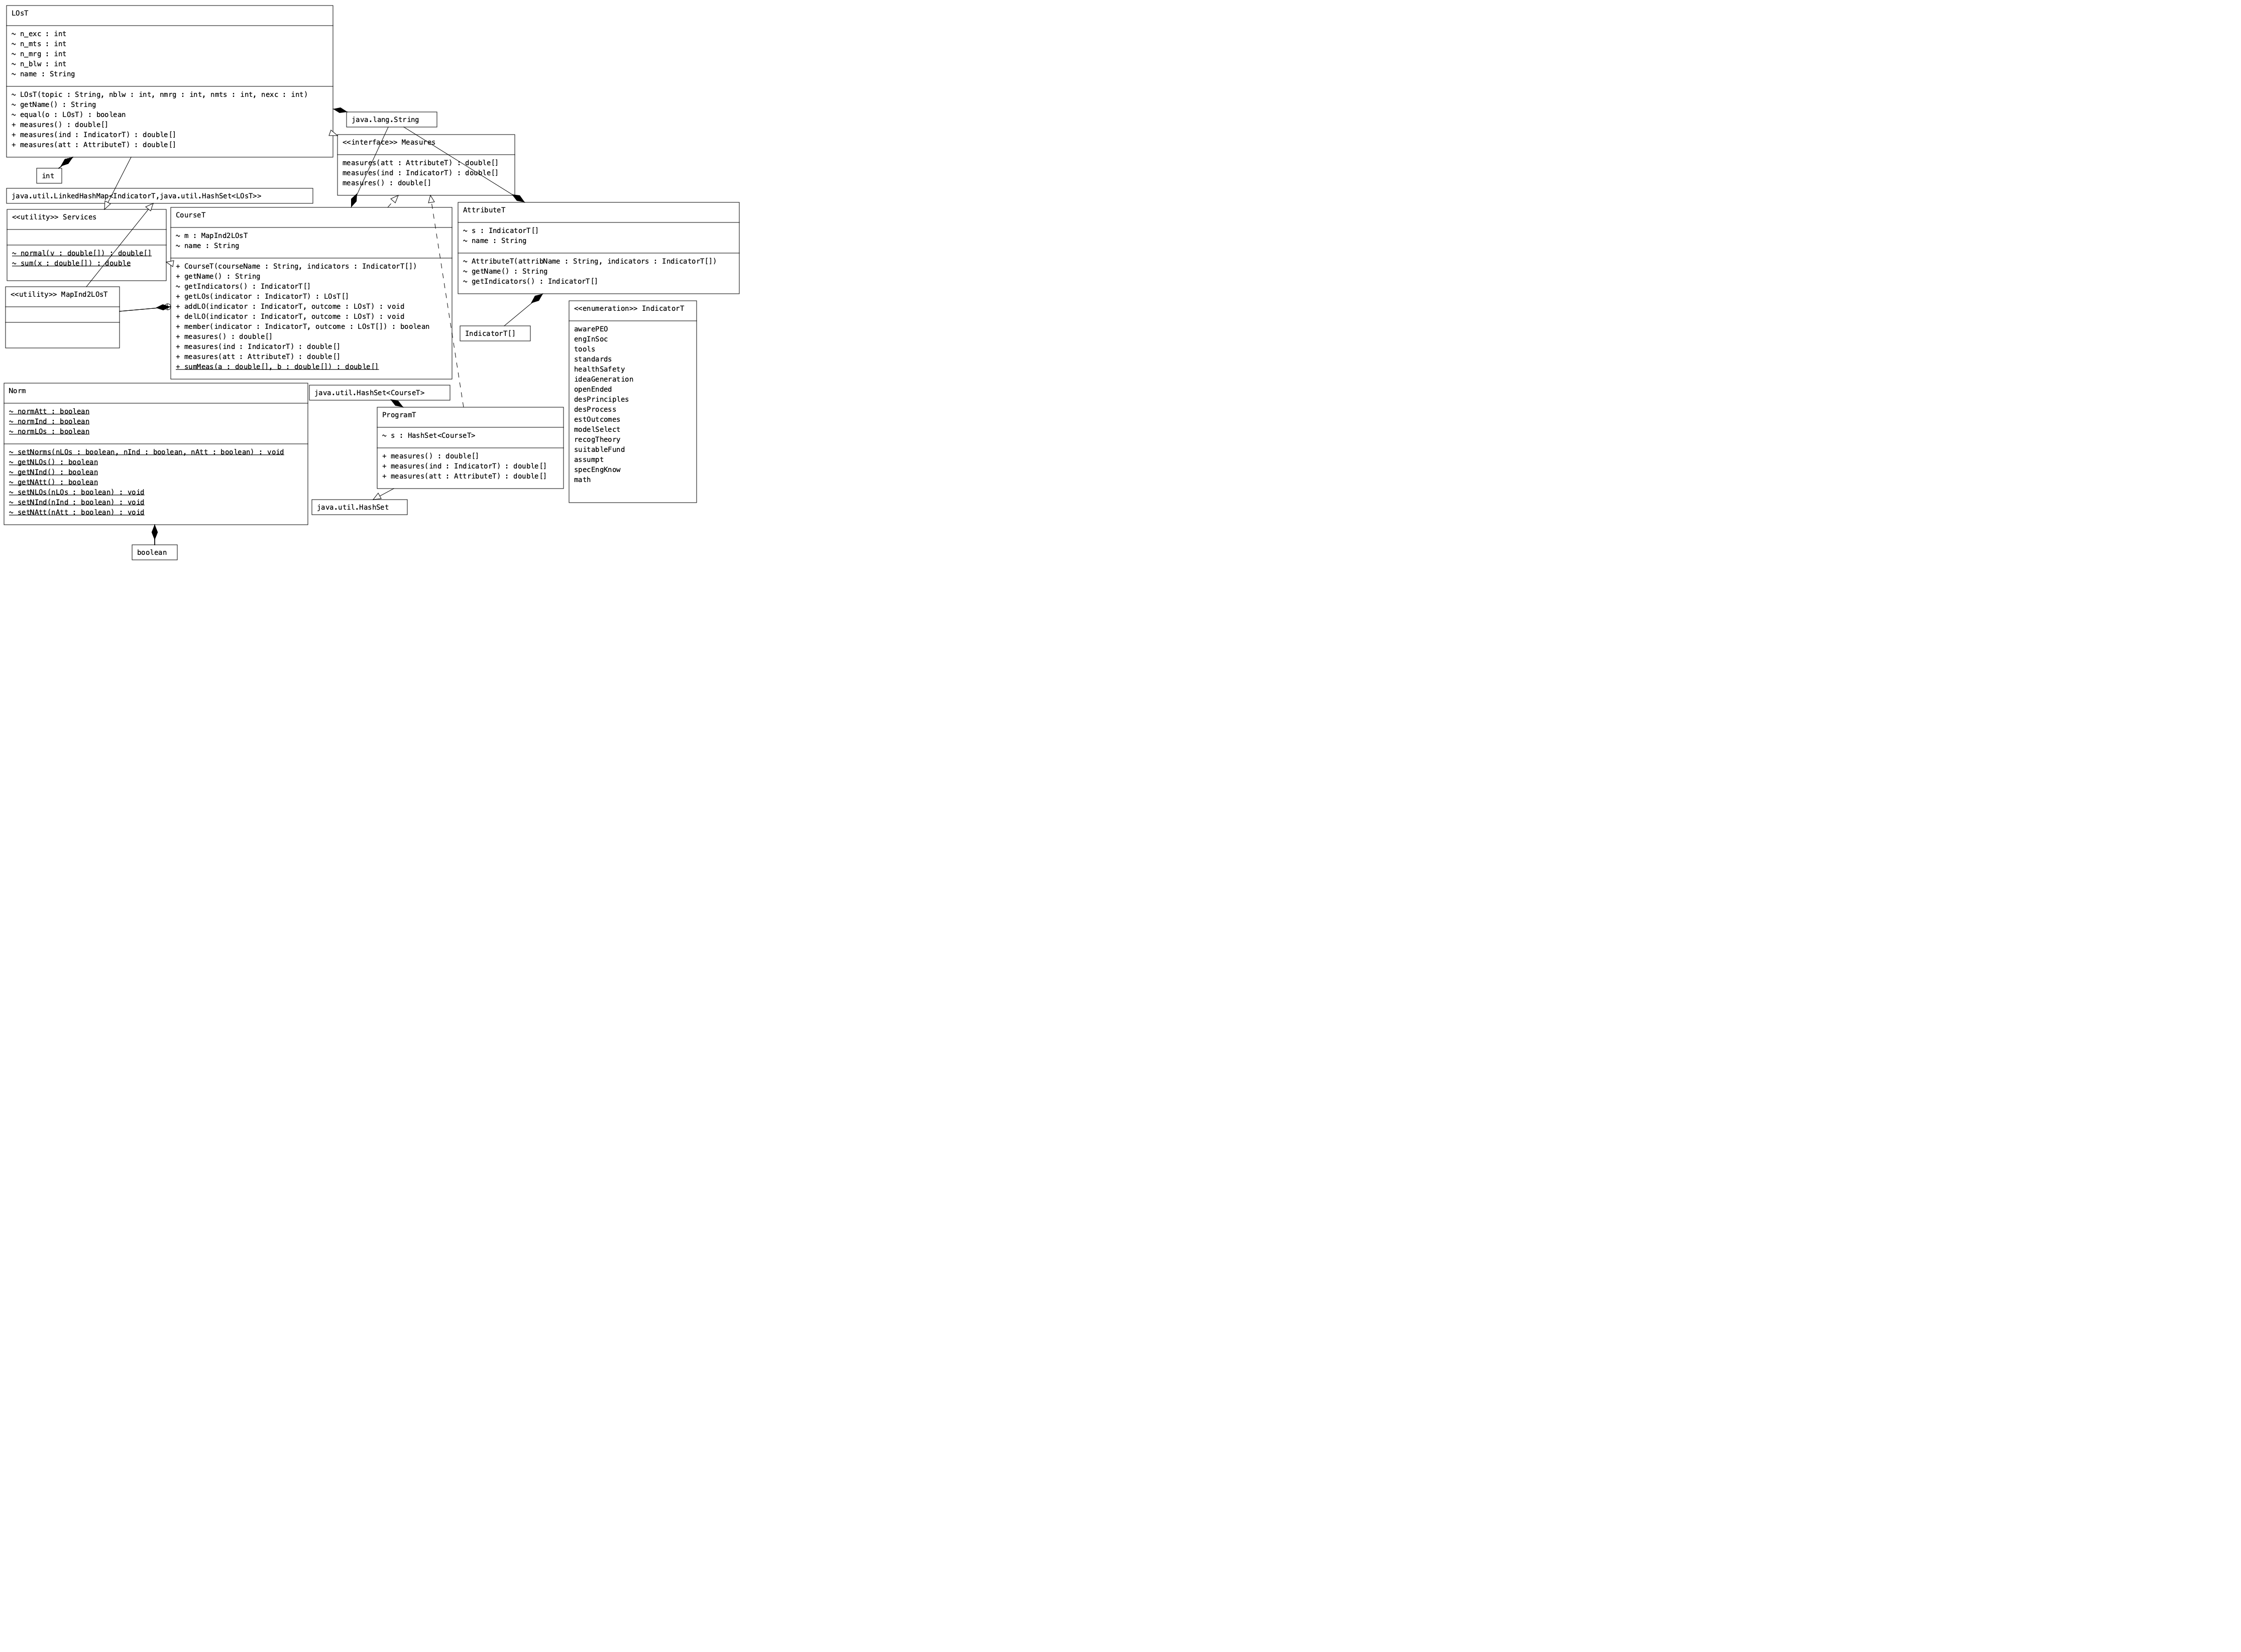
\includegraphics[width=50cm, height=50cm]{UML_final.png}


\end {document}
